\documentclass[11pt]{article}
\def\activityid{F05-FAC-v3}\usepackage[letterpaper,margin=.65in,top=.60in,bottom=.65in]{geometry}
\usepackage[T1]{fontenc}\usepackage[default]{sourcesanspro}
\usepackage{microtype,tikz,array,tabularx,fancyhdr,amsmath}\usepackage[hidelinks]{hyperref}
\usetikzlibrary{arrows.meta,calc}
\setlength{\parindent}{0pt}\setlength{\parskip}{7pt}\setlength{\headheight}{0pt}\setlength{\footskip}{26pt}\setlength{\emergencystretch}{2em}
\pagestyle{fancy}\fancyhf{}\renewcommand{\headrulewidth}{0pt}\renewcommand{\footrulewidth}{.4pt}
\fancyfoot[L]{\scriptsize Bellingham Math Circle / Week 5 / \activityid}\fancyfoot[R]{\scriptsize \thepage}
\definecolor{ink}{gray}{.12}\definecolor{soft}{gray}{.95}\color{ink}
\newcommand{\PageTitle}[2]{{\fontsize{10}{12}\selectfont\bfseries WEEK 5\quad TOWER LAB\hfill #1\par}\vspace{3pt}{\fontsize{26}{29}\selectfont\bfseries #2\par}\vspace{2pt}}
\newcommand{\Subhead}[1]{\par\vspace{3pt}{\large\bfseries #1}\par}
\newcommand{\RuleBox}[1]{\par\begingroup\setlength{\fboxsep}{8pt}\colorbox{soft}{\parbox{\dimexpr\linewidth-16pt\relax}{#1}}\endgroup\par}
\newcommand{\WriteBox}[2]{\par\textbf{#1}\par\vspace{2pt}\begin{tikzpicture}\draw[black!40,line width=.5pt] (0,0) rectangle (\dimexpr\linewidth-.5pt\relax,#2);\end{tikzpicture}\par}
\newcommand{\Code}[1]{\texttt{#1}}

\newcommand{\StudentHeader}[1]{{\fontsize{10}{12}\selectfont\bfseries Week 5 / Tower lab / #1\par}\vspace{10pt}}
\newcommand{\Problem}[2]{\par\vspace{4pt}\textbf{Problem #1:} #2\par}
\newcommand{\RecordBox}[2]{\par #1\par\vspace{2pt}\begin{tikzpicture}\draw[black!40,line width=.5pt](0,0)rectangle(\dimexpr\linewidth-.5pt\relax,#2);\end{tikzpicture}\par}

\hypersetup{pdftitle={Week 5: facilitator}}
\begin{document}
\PageTitle{FACILITATOR}{A city is a mathematical object}
\RuleBox{\textbf{Question:} How much information forces one arrangement? Children progress from a complete list to a uniqueness proof to a lower bound on clues. These are questions about permutations, Latin squares, and determining sets.}
\Subhead{Preparation and prerequisites}
Use snap cubes: six per youngest child, eighteen per middle child, forty for the upper child: \textbf{112 cubes}, plus a few for the launch. Prebuild towers if time is short. Numeral slips can record a second solution after the physical attempt. Start with page 1 for each child (seven student sheets). Keep continuation masters and this guide ready; copy the next page when the group needs it. Build on the tabletop or quick scrap-paper grids with one-inch cells. The smaller printed grids record solutions; they are not sized to hold every brand of cube.

K--1: compare heights/count to 3; no independent reading; recognize different orders. Middle: count to 3 and follow row/column rules; adult may read; distinguish an example from a complete list. Upper: count to 4; track constraints, cases, and uniqueness; no formal algebra. Extra: understand a 4-by-4 Latin square, coordinate labels, and a pigeonhole argument.
\Subhead{Launch}
Let towers be handled first. Show 2,1,3 from the left. Ask which towers a tiny person sees; touch each visible tower. Walk to the other end. Only after this introduce the separate city rule: every row and column uses each height once. A clue counts visible towers, not the first tower's height or the number of cubes.
\Subhead{A shared hour with seven children and two adults}
0--10: explore materials freely. 10--15: brief launch and rules. 15--35: main investigation. 35--40: movement/reset; preserve work. 40--55: continue or choose an optional proof. 55--60: share and tidy. This flexible default is our proposal, not a source prescription.

One adult stays with K,K,1. The organizer alternates middle and upper, leaving a concrete next attempt and returning for an explanation. In games keep two opposing sides and rotate a checker. Proof continuations need adult attention; pages are not a completion quota.

\textbf{K--1 stop:} Build all six skylines and describe their views. \textbf{Optional proof:} organize by first tower to show completeness; explain the impossible one-at-each-end view.

\textbf{Middle stop:} Build both top-clue cities and select one with the second clue. \textbf{Optional proof:} certify the list, then swap unseen rows/columns to rule out every one-clue puzzle.

\textbf{Upper stop:} Explain the complete five-clue case table. \textbf{Optional proof:} check all five deletion certificates and prove the three-clue alternative forces the same city. The computer's minimum claim is separate.

\newpage
\PageTitle{FACILITATOR}{Complete lists and minimum clues}
\Subhead{K--1: six skylines, not six unrelated puzzles}
The complete list (left count, right count) is: 123 (3,1), 132 (2,2), 213 (2,1), 231 (2,2), 312 (1,2), 321 (1,3). Fix the first tower: each of three choices leaves two orders. This proves completeness without factorial notation. One visible tower from both ends is impossible with distinct heights: the tallest would have to occupy both ends. Both 132 and 231 show two from each end.

The two 2-by-2 cities are 12/21 and 21/12. The top-row left clue 2 chooses the former. If row/column rules are too much, keep investigating rows; a complete skyline list is already substantial mathematics.
\Subhead{Middle: exactly two cities, then exactly one}
Top clue 3 forces first column 1,2,3. Top row is either 123 or 132. Column exclusions force the respective completions:
\begin{center}\begin{minipage}{.47\linewidth}\centering 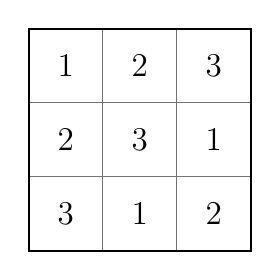
\begin{tikzpicture}[x=0.37in,y=0.37in]\draw[step=1,black!55] (0,0) grid (3,3);\draw[thick](0,0)rectangle(3,3);\node[font=\large]at(0.5,2.5){1};\node[font=\large]at(1.5,2.5){2};\node[font=\large]at(2.5,2.5){3};\node[font=\large]at(0.5,1.5){2};\node[font=\large]at(1.5,1.5){3};\node[font=\large]at(2.5,1.5){1};\node[font=\large]at(0.5,0.5){3};\node[font=\large]at(1.5,0.5){1};\node[font=\large]at(2.5,0.5){2};\end{tikzpicture}\end{minipage}\hfill\begin{minipage}{.47\linewidth}\centering 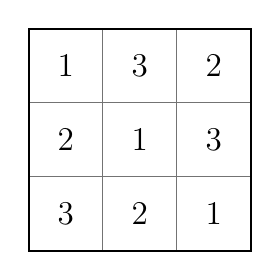
\begin{tikzpicture}[x=0.37in,y=0.37in]\draw[step=1,black!55] (0,0) grid (3,3);\draw[thick](0,0)rectangle(3,3);\node[font=\large]at(0.5,2.5){1};\node[font=\large]at(1.5,2.5){3};\node[font=\large]at(2.5,2.5){2};\node[font=\large]at(0.5,1.5){2};\node[font=\large]at(1.5,1.5){1};\node[font=\large]at(2.5,1.5){3};\node[font=\large]at(0.5,0.5){3};\node[font=\large]at(1.5,0.5){2};\node[font=\large]at(2.5,0.5){1};\end{tikzpicture}\end{minipage}\end{center}
The right clue 2 on row 2 keeps the first. Deleting that clue leaves both. Deleting only the top clue permits 123/231/312 and 312/231/123 (swap rows 1 and 3).

\textbf{A genuine minimum proof:} No single visibility clue can determine an entire 3-by-3 Latin square. If it sees a row, swap the two other rows; if it sees a column, swap the two other columns. The clue stays true and the square changes. Two clues suffice in our example, so the minimum over all uniquely solvable 3-by-3 visibility puzzles is two.
\Subhead{Hints and evidence}
K: fix the first tower and exchange the other two. Middle: point down the first column, then try both top rows. Ask what rules out another answer. Accept a complete physical case split; long written prose is unnecessary. If children only solve the city, ask for one clue deletion and an alternative, saving the minimum proof for conversation.

\newpage
\PageTitle{FACILITATOR}{A human certificate for five clues}
\Subhead{Upper: the unique solution}
Both the opening and the five-clue puzzle have rows \textbf{1234/2341/3412/4123}. Here is a small exhaustive argument for five clues. Bottom row starts with 4 and has right visibility 2, so 3 must be last. Only 4123 and 4213 remain. Keep both: the bottom clues alone do not rule either out; row 3 and row 2 do that next.

Row 3 has two views of 2. Its six possible rows are \textbf{1423, 2143, 2413, 3142, 3241, 3412}. Cross out candidates conflicting with the bottom row. The surviving pairs and possible row 2s are:
\begin{center}\renewcommand{\arraystretch}{1.3}\begin{tabular}{c|c|c}Bottom row&Row 3&Row 2 with right view 2\\\hline4123&3241&none\\4123&3412&2341\\4213&3142&none\end{tabular}\end{center}
Check the final column by listing row permutations avoiding the two entries already in each column, then testing the right view. The top row is forced by missing column heights. This proves uniqueness without trusting a solver.
\Subhead{Deleting clues: witnesses}
Deleting L3, L4, R2, R3, R4 gives \textbf{2, 2, 6, 12, 20} solutions respectively. L3 means the left clue on row 3. One alternative per deletion proves necessity:
\begin{center}\small\renewcommand{\arraystretch}{1.35}\begin{tabular}{c|l}Delete&Alternative city, top row first\\\hline L3&1234 / 3412 / 2341 / 4123\\L4&1234 / 4123 / 3412 / 2341\\R2&1324 / 2431 / 3142 / 4213\\R3&1324 / 3142 / 2431 / 4213\\R4&1234 / 2143 / 3412 / 4321\end{tabular}\end{center}
On optional upper page 4, check each certificate is Latin, keeps all four retained clues, and differs from the target. Restoring the clue before the next deletion keeps the five arguments separate. The five-clue set is \textbf{minimal}, but it is \textbf{not minimum}: left clues 4,3,2 on rows 1,2,3 uniquely determine this same target. First row is 1234. The rows with left view 3 are 1243,1324,1342,2134,2314,2341; all but 2341 repeat a column entry. With rows 1 and 2 fixed, the possible row 3s are 3412 and 4123; only 3412 has left view 2. The last row is forced.

The script exhaustively verifies that three is the minimum \emph{for this target city among subsets of its 16 perimeter clues}. That computation is not a proof that every 4-by-4 city needs three. For children, the concrete three-clue alternative already disproves the claim that minimal means minimum.

\newpage
\PageTitle{FACILITATOR}{Trades, bounds, and research}
\Subhead{Extra: a lower bound with an escape move}
Each bold block has form \(ab/ba\). Exchanging \(a,b\) inside it preserves the multiset in each affected row and column. With at most three entry clues, one of four disjoint blocks has no clue. Switch it: a distinct Latin square keeps every given entry. Thus at least four \emph{entry} clues are necessary for this square.

Hitting these four blocks is not sufficient. Clues at (1,1), (1,3), (3,1), (3,3) leave rows 2 and 4 unclued; swapping those rows keeps all four clues. Any uniquely determining set must meet \emph{every} trade. Conversely, the changed cells in any alternative completion form a trade; hitting every such trade rules out alternatives.

\textbf{Keep clue types separate:} Previous pages use outside visibility clues; the extra uses fixed entries. Bounds do not transfer automatically.
\Subhead{Where the mathematics goes}
Undergraduate combinatorics studies permutations, Latin squares, constraint satisfaction, and hitting sets. Joy Morris's \href{https://opentext.uleth.ca/Combinatorics/ch_Latin-squares.html}{\emph{Combinatorics}, chapter on Latin squares} develops Latin-square structure; our visibility questions add a different constraint system.

Hatami and Qian, \href{https://arxiv.org/html/1606.00032}{\emph{Teaching dimension, VC dimension and critical sets for Latin squares}} (2016), \S1 and Theorem 1.2, study sets of \emph{entries} determining a square and prove a quadratic lower bound for sufficiently large orders. Our trade argument is a small instance of the question, not their asymptotic theorem. The paper states a sharper conjecture; no current open-status claim is needed here.
\Subhead{Teaching sources and returning children}
JRMF \emph{Skyscrapers Teaching Guide}, PDF pp. 1--4: physical viewpoints, city rules, and reasoning; pp. 13--14: blank boards. Our clue instances and investigations extend that format. \emph{Math Circle by the Bay}, printed pp. ix--x: manipulatives, extra challenges, and themes at different depths. Lowell Handout 2.1--2.2 seating constraints are related prior material, not evidence children have solved these cities.

Use F05-K-v3/M-v3/U-v3/X-v3. Prepared, not recorded as taught. Save trade classification, Latin transversals, and larger skyline recurrences for later years. Rebuild with \texttt{build.sh}; \texttt{plans/verify-week-05.py} checks the finite claims independently of the explanations.


\newpage
\PageTitle{FACILITATOR}{Using the revised sequence}
\Subhead{Classroom evidence and this new proposal}
Revision v3, September 27, 2026: \textbf{unpiloted}. Week 1 feedback reported too little work before new ideas, unclear next actions, and simultaneous adult demand. It did not report a Week 5 trial. These revisions apply that guidance by giving each viewpoint several attempts and each later representation a job. Preserve children's actual records; do not equate an unfinished packet with a failed session.
\Subhead{Launch and handoff}
After handling the cubes, gather everyone around towers 2,1,3. Touch the towers visible from each end; record 2,1,3 left to right and write its two view counts. Then change to 1,3,2 and let a child check. Distribute first pages only after children can make and record that action. Demonstrate the row/column city rule locally when a group reaches a grid; the K group can spend the whole session on rows.

K pages 1--2 provide repeated views and a complete list. Problem 1 has views (2,1), Problem 2 has (2,2). Problem 3 accepts 123 for three; 312 or 321 for one; 132,213,231 for two. Problem 6 has no solution; preserve two unsuccessful attempts before discussing the tallest-at-both-ends argument. Page 3's city rule is a separate reserve.

Middle page 1's four rows have view pairs (3,1), (2,1), (2,2), (1,3). Any Latin city and any whole-row swap meet Problem 2. Pages 2--3 stage the top clue, a second clue, and a deletion, with separate grids. Stop after the two top-clue cities if comparison still needs time. Ask the completeness and unseen-row/column-swap proofs orally only after the children have built the alternatives.

Upper page 1's row views are (2,2), (2,2), (1,2), (1,2). Page 2 isolates possible rows before page 3 organizes them into cases. The complete lists and table on this guide's page 3 answer Problems 4--7. Pages 4--5 are optional clue investigations. The covered-clue views for Problem 9 are respectively \textbf{3,3,3,3,4}; each violates the restored target clue while retaining the other four. A smaller construction and a lower bound are different claims. Preserve the minimal/minimum discussion in conversation after the checked deletion records and three-clue construction.
\Subhead{Extra and practical pacing}
Extra page 1 tests four individual switches before entry clues appear on page 2. For any three circled cells, at least one of four blocks is untouched; any such switch works. For Problem 4, use the original city and \textbf{1234/4321/3412/2143}, obtained by swapping rows 2 and 4. Each has the four fixed entries. Invite the four-block lower-bound and every-trade arguments from page 4 of this guide after these concrete checks.

Allow 15--35 minutes for first attempts, a 35--40 movement break, and 40--55 for the current idea or one selected continuation. Keep 55--60 for sharing. Do not start two adult-dependent proof discussions together. Offer pointing, building, or dictation for every recording task.
\Subhead{Record after use}
Record exact problem numbers attempted, viewpoint/row-rule errors, any instructions needing repeated adult rescue, what children chose to continue, and explanations actually given. Keep observations separate from hypotheses and proposed revisions. Source support: \emph{Math Circle by the Bay}, pp. ix--x; Rozhkovskaya, Lessons 3,7,8, ``At the lesson.'' These support flexible pacing and representation after attempts; the exact sequence is our adaptation.

\end{document}
